\documentclass[a4paper,12pt]{article}

\usepackage[utf8x]{inputenc}
\usepackage[italian]{babel}
\usepackage{graphicx}

%opening
\title{Fisica dei Sistemi Complessi\\Relazione di progetto\\3D Network Visualizator}
\author{Giacomo Benvenuti\\Enrico D'Angelo\\Fabrizio Nuzzo}
\date{}

\begin{document}

\maketitle

\begin{abstract}
La visualizzazione dei dati \`e lo studio della rappresentazione visuale dei dati stessi, lo scopo principale \`e quello di comunicare le informazioni contenute nei dati in maniera chiara ed efficace. Per trasmettere le informazioni sia l'estetica che la funzionalità della visualizzazione devono andare di pari passo, in modo da fornire la comprensione delle informazioni contenute in un dataset altrimenti complesso da comprendere. Lo scopo fondamentale della visualizzazione dei dati \`e quindi la comunicazione degli aspetti chiave del dataset in una maniera più intuitiva.

Il progetto svolto ha lo scopo di visualizzare le interazioni che avvengono nei diversi istanti tra i nodi di una rete. 3D-Network-Visualizator visualizza queste interazioni in maniera grafica. I nodi che compongono la rete sono disposti in uno spazio tridimensionale secondo le loro coordinate. Le interazioni vengono visualizzate come degli archi che vanno da un nodo all'altro dando una diversa ampiezza all'arco in base alla frequenza dell'interazione, per meglio capire a colpo d'occhio l'importanza relativa delle diverse interazioni. Infine gli istanti scorrono su una linea temporale dando la possibilità di visualizzare come in un video i cambiamenti che avvengono nelle interazioni tra i diversi nodi.
\end{abstract}

\section{Il Problema}
L'uomo per sua natura ha una spiccata capacit\`a d'analisi critica ma questa deve essere supportata da una chiara ed appropriata visualizzazione dei dati.

Osservando direttamente un dataset che rappresenta una rete e le interazioni che avvengono tra i suoi nodi, anche se di dimensioni modeste, non \`e immediato rispondere a domande quali: “quali sono le interazioni che avvengono?”, “quali nodi sono quelli con maggiori o minori interazioni?”, “esistono delle interazioni ricorrenti tra certi nodi?” Che sono solo alcune delle domande di interesse per chiunque si trovi ad analizzare un dataset di questo tipo.

\subsection{Una possibile soluzione}
Un modo semplice per rappresentare una rete consiste nell'utilizzare una tabella con l'elenco di tutto i nodi della rete riportato sia nelle righe che nelle colonne. In questo modo nella cella che incrocia due nodi viene riportato il valore che rappresenta l'interazione avvenuta tra quei due nodi. Una tabella pu\`o per\`o rappresentare lo stato delle interazioni della rete in un solo istante, per poter osservare le interazioni nel tempo occorre quindi utilizzare una tabella per ogni istante.

\subsection{Considerazioni}
Nonostante questo approccio sia molto semplice, non e' auspicabile perché inefficiente dal punto di vista computazionale e della leggibilità dei risultati; Se per esempio volessimo rappresentare le interazioni che avvengono in ogni istante di tempo che non coinvolgono tutte le coppie di nodi, le tabelle risulterebbero sparse, perci\`o viene utilizzata una gran quantità di memoria per memorizzare in realtà una piccola quantità di informazione. Questo problema viene ulteriormente peggiorato quando la rete contiene un gran numero di nodi.

\section{Specifiche di funzionamento}
3D-Network Visualizator come il nome lascia intendere, un visualizzare grafico 3D delle interazioni che avvengono tra i nodi di una rete.
\begin{itemize}
 \item Le informazioni di input, devono essere elaborate prima della visualizzazione grafica di quest'ultime.
 \item L'altezza dell'arco dipende dalla frequenza (cio\`e il valore dell'interazione).
 \item Deve essere possibile capire la velocità con cui i nodi comunicano
 \item Deve essere possibile cambiare l'angolazione della visualizzazione
 \item Deve essere possibile partizionare la rete per analizzare una parte di essa
 \item La visualizzazione  deve essere personalizzabile tramite varie opzioni
 \item Deve essere possibile variare il tempo di visualizzazione di un istante
\end{itemize}
 
\section{Tecnologie utilizzate}
Per la realizzazione di questo progetto sono state utilizzate diverse tecnologie:
\begin{description}
 \item[Processing:] \`e una libreria di sviluppo e un linguaggio di programmazione open source, derivato da Java. Esso viene incontro a necessità di utilizzo più specifico dal punto di vista grafico. Le molteplici possibilità della libreria combaciano perfettamente con le nostre aspettative di rappresentazione grafica del progetto. Processing viene oggi utilizzato da studenti, artisti, designers, ricercatori e obbisti per produrre prototipi e prodotti finiti di livello professionale. Processing \`e stato inizialmente sviluppato da Ben Fry e Casey Reas nel 2001 mentre erano entrambi studenti sotto la supervisione di John Maeda al MIT Media Lab. Ulteriore sviluppo di Processing ha avuto luogo all'Interaction Design Institute Ivrea, Carnegie Mellon University, e alla UCLA, dove Reas \`e capo del Dipartimento di Design | Media Arts. Miami University, Oblong Industries, e la fondazione Rockefeller hanno contribuito finanziando il progetto.
 \item[XML:] (eXtensible Markup Language). Per rappresentare l'input \`e necessario un formato che memorizzi solo le informazioni reali, cio\`e solo l'elenco delle interazioni avvenute in un dato istante. XML \`e un linguaggio di markup che permette di definire dati strutturati facilmente leggibili dall'uomo e facilmente analizzabili da un computer. L'utilizzo del formato XML per definire l'input del programma di visualizzazione della rete permette di memorizzare in modo efficiente solo le informazioni necessarie, rendendo, tra l'altro, la loro analisi più semplice da un punto di vista algoritmico.
 \item[Java]  linguaggio di programmazione orientato agli oggetti, indipendente dalla piattaforma.
\end{description}
        
\section{Funzioni Implementate}
 
\subsection{creazione di una network history}
3D network visualizator permettere di creare una simulazione  personalizzata, questa funzione \`e disponibile nel pannello principale del programma, o tramite il menu 
File -> crea una nuova rete.
i passi sono principalmente quattro:
\begin{enumerate}
 \item Inserire nel campo “Nome della rete” il nome che identificherà il nostro file;
 \item inserire nel campo “Nome del nodo” il nome del nodo che farà parte del nostro network nei campi “coordinate:” il valore delle coordinate X,Y,Z.
 \item Inserire le varie interazioni tra i nodi tramite i campi: 
  \begin{itemize}
   \item istante (il momento in cui vogliamo che i nodi iniziano l'interazione ). 
   \item campi “nodo sorgente:” e “nodo destinatario:” i nomi dei nodi interessati all'interazione (\`e possibile far partecipare più nodi a un'interazione).
   \item campo “Tempo:” il tempo che i nodi saranno impegnati nell'interazione.
   \item campo “Frequenza:” con quale frequenza i nodi si scambieranno messaggi.
  \end{itemize}
 \item tramite l'opzione “Usa sfera come struttura” \`e possibile utilizzare una sfera invece del classico piano.
\end{enumerate}

\subsection{importare una rete in formato xml}
Tramite il menu File -> “Importa una nuova rete” \`e possibile caricare una file precedentemente creato tramite il pannello “crea network” o tramite il “generatore di reti random”.

\begin{figure}[htb!]
 \begin{center}
  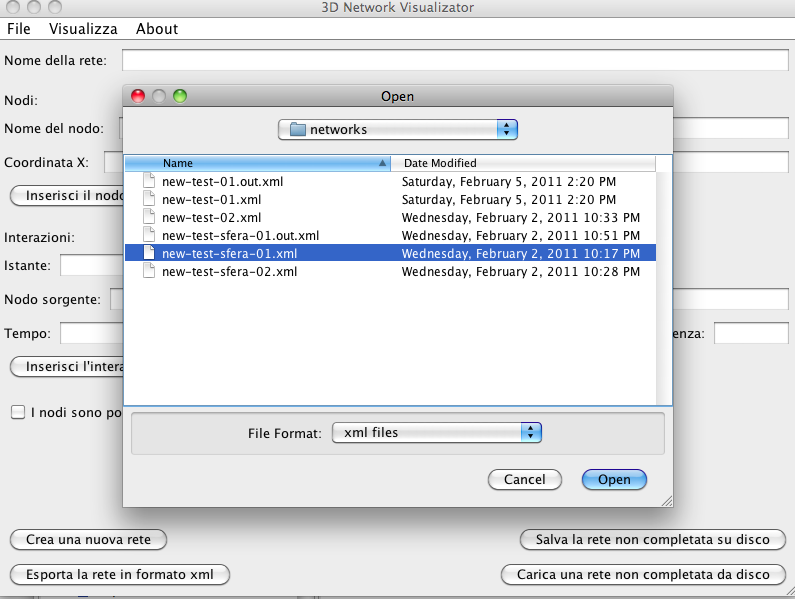
\includegraphics[width=\textwidth]{images/image0.png}
 \end{center}
 \caption{File dialog per importare una nuova rete.}
 \label{fig:importnetwork}
\end{figure}
 
Una volta importato il file, il programma visualizzerà il pannello di processing con la nostra struttura di base (piano o sfera) dove verranno posizionati i vari nodi durante una breve animazione introduttiva. Finita l'animazione \`e possibile far partire la simulazione tramite il tasto “play” posizionato nella barra dei comandi (\figurename~\ref{fig:slider}). 
In qualsiasi momento possibile fermare la simulazione tramite il tasto “pause” (\figurename~\ref{fig:slider}) per analizzare le interazioni di quel momento.
Lo slider posto sempre nella barra in basso (\figurename~\ref{fig:slider}) mostra l'avanzamento della simulazione in percentuale. 
Tramite il campo situato a fianco lo slider \`e possibile cambiare la durata di un istante, questa opzione \`e molto utile per soffermarsi sulle interazione che avvengono in ogni  istante.
 
\begin{figure}[htb!]
 \begin{center}
  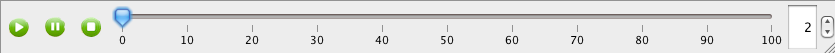
\includegraphics[width=\textwidth]{images/image1.png}
 \end{center}
 \caption{Slider per controllare l'animazione delle interazioni.}
 \label{fig:slider}
\end{figure}
 
\subsection{Opzioni di Visualizzazione}
Tramite il menu Visualizza \`e possibile accedere a diverse opzioni di visualizzazioni tra cui:
1. Visualizza spazio 3d di riferimento (attiva di default) tramite questa opzione \`e possibile nascondere la griglia di riferimento dell'animazione dove sono posizionati i nodi. Questa opzione \`e utile per ridurre al minimo gli elementi presenti nel riquadro.
2. Visualizza solo archi entranti (disattivata di default) questa opzione \`e molto utile se  vogliamo visualizzare solo le connessioni e il traffico in ingresso; questa opzione \`e utilizzabile in accoppiata alla funzione partizione in modo da visualizzare solo le connessioni e il traffico in ingresso  di determinati nodi.
3. Visualizza gli archi di tutti i nodi (attiva di default)   Questa opzione permette di nascondere in qualsiasi istante gli archi della rete, utile per visualizzare la posizione dei nodi sulla griglia; questa opzione \`e utilizzabile in accoppiata alla funzione partizione.
 
 
 
\subsection{Interazione con una partizione della rete}
Durante i primi test della nostra applicazione abbiamo notato che era difficoltoso concentrare l'attenzione su una ristretta cerchia di nodi, appunto una  partizione della rete. L'attività della rete cambia ogni istante e la possibilità che le connessioni  interessino tutti  i nodi non \`e remota. Uno scenario del genere \`e sicuramente utile per avere un quadro completo della situazione  in un dato istante ma se la nostra analisi \`e rivolta soltanto a determinati nodi tutte le altre interazioni tra i nodi della rete risultano superflue.

\begin{figure}[htb!]
 \begin{center}
  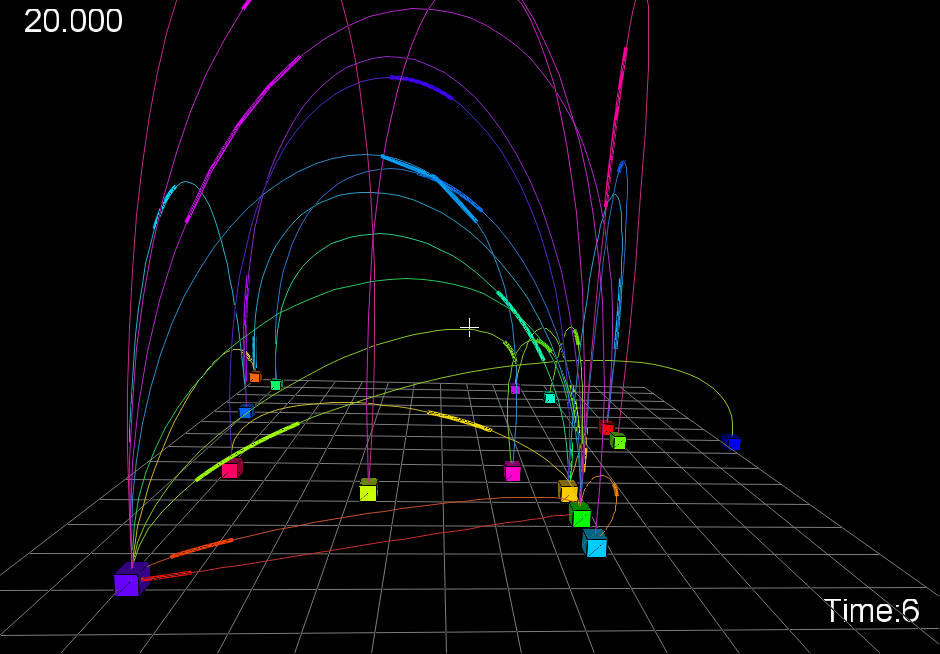
\includegraphics[width=\textwidth]{images/image2.png}
 \end{center}
 \caption{esempio di visualizzazione senza partizione.}
 \label{fig:slider}
\end{figure}
 
Per ovviare a questo problema \`e stata implementata la funzione partizione; 
Questa funzione \`e disponibile  in qualsiasi momento dell'animazione; per utilizzarla basta portarsi con il cursore sul nodo/i che ci interessano e selezionarli premendo i tasto “ctrl”.

\begin{figure}[htb!]
 \begin{center}
  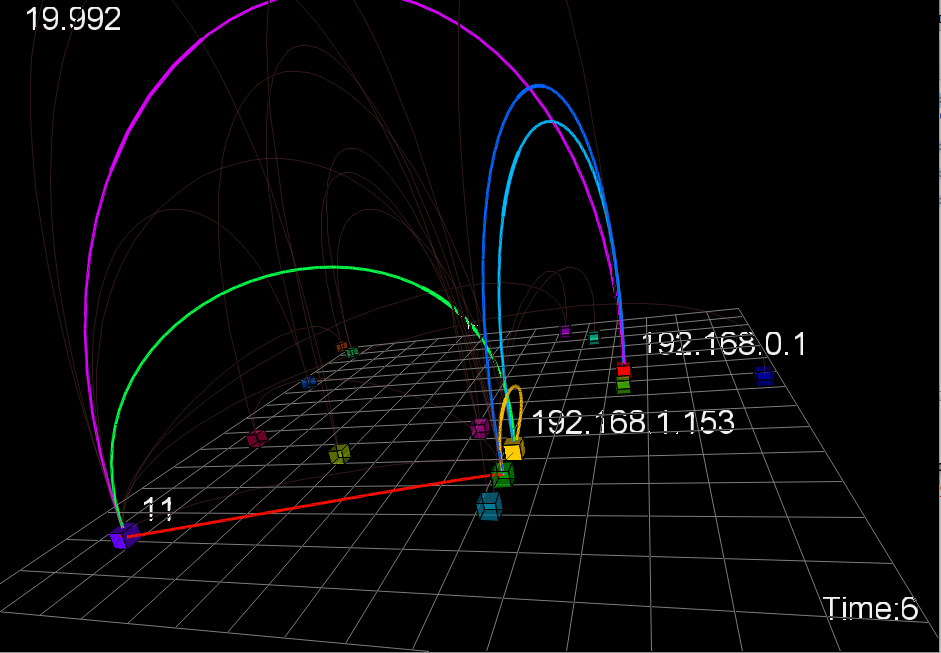
\includegraphics[width=\textwidth]{images/image3.png}
 \end{center}
 \caption{esempio di visualizzazione con  partizione.}
 \label{fig:slider}
\end{figure}
 
In questo screenshot possiamo notare come la funzione partizione faciliti l'analisi di questa parte del network formata da 3 nodi nell'istante 6 
 
\subsection{Tipologie di struttura}
 
\subsubsection{Piano}

\begin{figure}[htb!]
 \begin{center}
  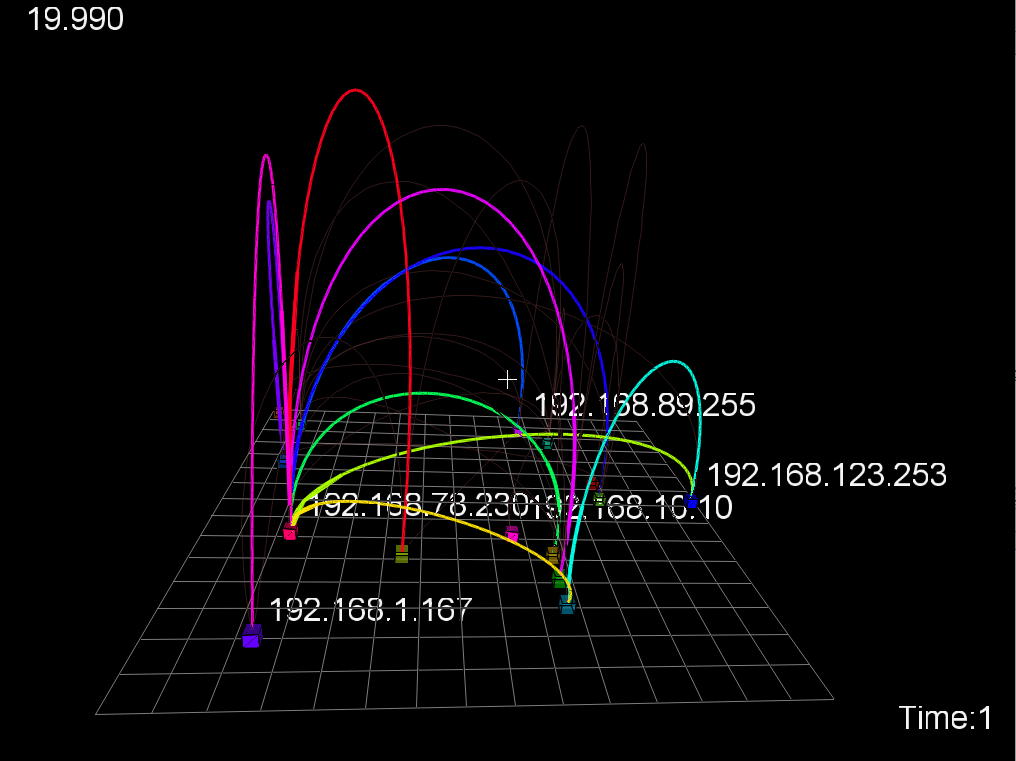
\includegraphics[width=\textwidth]{images/image4.png}
 \end{center}
 \caption{esempio di visualizzazione con  partizione.}
 \label{fig:slider}
\end{figure}

\subsubsection{Sfera}

\begin{figure}[htb!]
 \begin{center}
  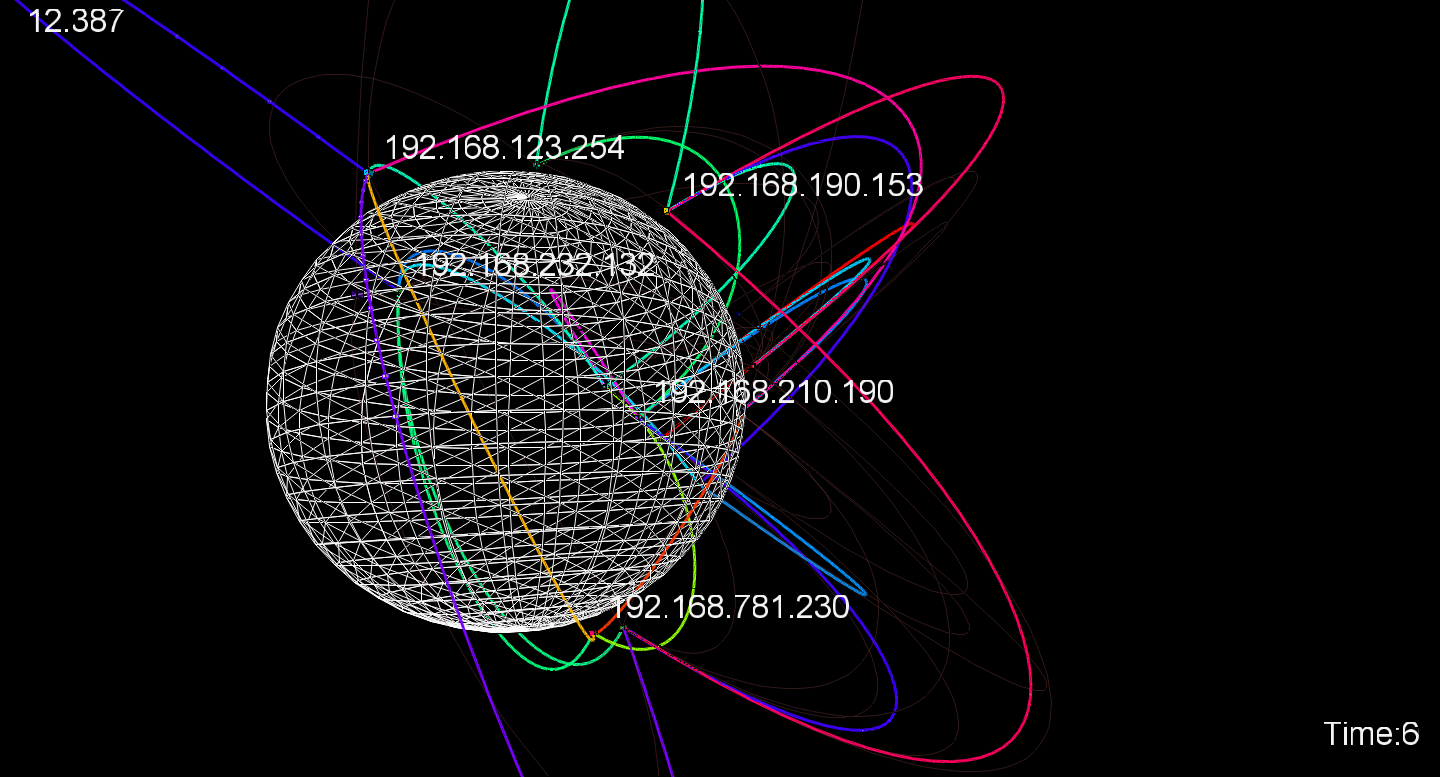
\includegraphics[width=\textwidth]{images/image5.png}
 \end{center}
 \caption{esempio di visualizzazione con  partizione.}
 \label{fig:slider}
\end{figure}
 
\section{Il dataset}
Il tipo di dataset che viene visualizzato contiene tutte le informazioni che riguardano i nodi che compongono la rete, e istante per istante, tutte le interazioni che avvengono tra i nodi.
Gli attributi che riguardano i nodi sono:
\begin{description}
 \item[l'identificativo] \`E un identificativo numerico che viene utilizzato all'interno del dataset per indicare uno specifico nodo. Ogni nodo possiede un identificativo univoco.
 \item[l'etichetta] L'etichetta svolge circa lo stesso ruolo dell'identificativo ma \`e più adatta per essere memorizzata dalle persone. gli identificativi servono al software per distinguere e identificare i diversi nodi, per questo motivo sono degli indici numerici. Per una persona \`e invece molto più facile memorizzare degli identificativi alfanumerici, e questo \`e lo scopo delle etichette. Inoltre quando i nodi rappresentano delle entita fisiche esistenti, come ad esempio delle città, \`e utile che le label rispecchino il nome di tale entità al fine di aiutare la comprensione del fenomeno. L'etichetta di un nodo non deve necessariamente essere univoca.
 \item[coordinate] Sono le coordinate cartesiane dei nodi.
\end{description}

Gli attributi che riguardano le interazioni sono:
\begin{description}
 \item[la sorgente] \`E l'identificativo del nodo da cui ha origine l'interazione.
 \item[l'obiettivo] \`E l'identificativo del nodo obiettivo dell'interazione.
 \item[quantità] Rappresenta la quantità del flusso che costituisce l'interazione. Cosa sia effettivamente il flusso che costituisce l'interazione dipende dal tipo di rete in esame. Pu\`o per esempio trattarsi di pacchetti scambiati da diversi elaboratori collegati via rete, o di automobili che si spostano da un luogo ad un altro.
 \item[frequenza] \`E la frequenza che caratterizza l'interazione.
\end{description}

Le informazioni che riguardano le interazioni sono naturalmente suddivise per istanti. Anche gli istanti hanno degli attributi:
\begin{description}
 \item[valore] \`E l'identificativo dell'istante. Gli identificativi degli istanti devono essere univoci e consecutivi.
 \item[etichetta] Anche in questo caso le etichette servono per meglio comprendere il fenomeno. Le etichette possono infatti rispecchiare il tempo fisico, l'ora, in cui sono state prese le misurazioni che costituiscono le informazioni riguardanti le interazioni.
\end{description}
 
\subsection{Il file network XML}
 
L'input del nostro visualizzatore \`e un file che contiene la descrizione della topologia di una rete e le interazione che avvengono tra i suoi nodi. Come formato del file di input abbiamo scelto l'XML per diversi motivi. In primo luogo per la facilità con cui pu\`o essere processato da un calcolatore. In secondo luogo per la sua portabilità su diverse piattaforme e linguaggi di programmazione, in questo modo lo stesso file di input pu\`o essere utilizzato facilmente anche da altri software scritti in altri linguaggi di programmazione per altre piattaforme software. Infine per la sua caratteristica di essere facilmente leggibile anche dall'uomo.
Il pricipale punto a sfavore di questo formato \`e la scarsa compattezza, nel senso che oltre alle informazioni relative alla rete il file contiene anche molte meta-informazioni che servono appunto per facilitare l'elaborazione del file e facilitarne la sua leggibilità. Questo significa che per file di input che rappresentano reti di grandi dimensioni, ad esempio con migliaia di nodi e centinaia di interazioni, molto spazio per la memorizzazione del file su disco sarà occupato dalle meta-informazioni. In questi casi un formato binario sarebbe stato sicuramente più compatto, ma avrebbe perso tutte le caratteristiche positive elencate sopra.
 
Qui di seguito viene riportato un file di input di esempio:
\begin{verbatim}
<?xml version="1.0" encoding="UTF-8"?>
<network>
 <static-data>
   <network-name>new-test-02</network-name>
   <nodes-list>
     <node id="0" label="192.168.0.1" x="2" y="0" z="6" />
     <node id="1" label="192.168.0.2" x="3" y="0" z="8" />
   </nodes-list>
   <flat>true</flat>
 </static-data>
 <dynamic-data>
   <instant value="0" label="0">
     <interaction source="1" target="0" quantity="1" frequency="0.6080425" />
   </instant>
   <instant value="1" label="1">
     <interaction source="1" target="0" quantity="8" frequency="1.31866568" />
   </instant>
 </dynamic-data>
</network>
\end{verbatim}

La struttura del file di input \`e divisa in due parti principali:
\begin{description}
 \item[static-data:] Questa parte contiene le informazioni statiche della rete, cio\`e la sua topologia, \`e composta dai seguenti elementi:
 \begin{itemize}
  \item network-name: il nome della rete
  \item nodes-list: l'elenco dei nodi presenti nella rete
  \item flat: indica se la rete deve essere visualizzata in uno spazio piano o sferico
 \end{itemize}
Ogni nodo in nodes-list \`e descritto con i seguenti attributi:
 \begin{itemize}
  \item id: \`e l'identificativo univoco del nodo
  \item label: \`e l'etichetta del nodo
  \item x, y e z: sono le coordinate del nodo.
 \end{itemize}
 \item[dynamic-data:] Questa parte contiene tutte le informazioni dinamiche della rete, cio\`e le interazioni che avvengono tra i suoi nodi. \`E strutturata come una lista di istanti. Ogni istante \`e strutturato come una lista di interazioni. Ogni interazione \`e descritta con i seguenti attributi:
 \begin{itemize}
  \item source: \`e l'identificativo del nodo dal quale parte l'interazione
  \item target: \`e l'identificativo del nodo obiettivo dell'interazione
  \item quantity: rappresenta la quantità di dati scambiati durante l'interazione
  \item frequency: \`e la frequenza dell'interazione
 \end{itemize}
\end{description}

\section{Conclusioni }
 
Lo studio e l'implementazione del programma 3D Network Visualizator ci ha dato la possibilità di scoprire i vantaggi derivati da una efficace ed adatta visualizzazione dei dati. Spesso per effettuare analisi non basta avere statistiche dettagliate e indici ricavati da grandi quantità di dati per il semplice motivo che viene a mancare una visione d'insieme che potrebbe portare un risultato d'analisi inaspettato.
Inizialmente il nostro dominio applicativo erano le reti di calcolatori dislocate geograficamente che scambiano pacchetti di dati. Il dominio in questione per quanto pu\`o essere banalmente descrivibile per esempio tramite un grafico bidimensionale, esclude alcune informazioni che potrebbero essere importanti in caso di analisi approfondite. Una fra tutte la frequenza con cui i nostri ipotetici calcolatori si scambiano pacchetti; come rendere visibile questa informazione? L'introduzione della terza dimensione \`e stata essenziale per poter aggiungere elementi. 
Prendendo in esempio la frequenza con cui i nodi si scambiano i pacchetti, la nostra soluzione \`e stata di curvare il link in modo da creare un arco in relazione all'aumento della frequenza di comunicazione. Questo tipo di approccio \`e risultato di sicuro impatto per avere un idea dei nodi che hanno un scambio maggiore dei pacchetti nella rete in un dato istante. 

\end{document}